\documentclass[a4paper,10pt]{article}

\usepackage[utf8]{inputenc}
\usepackage{t1enc}
\usepackage[spanish]{babel}
\usepackage[pdftex,usenames,dvipsnames]{color}
\usepackage[pdftex]{graphicx}
\usepackage{amsmath}
\usepackage{hyperref}
\usepackage{amsfonts}
\usepackage{amssymb}
\usepackage{listings}
\lstset{language=C}
\lstset{showstringspaces=false}
\lstset{basicstyle=\ttfamily,}

\begin{document}


\renewcommand{\lstlistingname}{C\'odigo Fuente}
\lstloadlanguages{Octave} 
\lstdefinelanguage{MyPseudoCode}[]{Octave}{
	deletekeywords={beta,det},
	morekeywords={repmat}
} 
\lstset{
	language=MyPseudoCode,
	stringstyle=\ttfamily,
	showstringspaces = false,
	basicstyle=\footnotesize\ttfamily,
	commentstyle=\color{gray},
	keywordstyle=\bfseries,
	numbers=left,
	numberstyle=\ttfamily\footnotesize,
	stepnumber=1,                   
	framexleftmargin=0.20cm,
	numbersep=0.37cm,              
	backgroundcolor=\color{white},
	showspaces=false,
	showtabs=false,
	frame=l,
	tabsize=4,
	captionpos=b,               
	breaklines=true,             
	breakatwhitespace=false,      
	mathescape=true
}
\begin{titlepage}
        \thispagestyle{empty}
        \begin{center}
                
\includegraphics{./images/itba.jpg}
                \vfill
                \Huge{Sistemas Operativos}\\
                \vspace{1cm}
                \huge{Trabajo Práctico Especial}\\
        \end{center}
        \vspace{2cm}
        \large{
                \begin{tabular}{lcrc}
                        \textbf{Alvaro Crespo} & & 50758 & \ \ \texttt{acrespo@alu.itba.edu.ar}\\
                        \textbf{Juan Pablo Civile} & & 50453 & \ \ \texttt{jcivile@alu.itba.edu.ar}\\
                        \textbf{Darío Susnisky} & & 50592 & \ \ \texttt{dsusnisk@alu.itba.edu.ar}\\
                        \\ 
                \end{tabular}
        }
        \vfill
        \flushright{24 de Octubre del 2011}
\end{titlepage}

\setcounter{page}{1}

\tableofcontents
\newpage
\section{Introducción}
El trabajo práctico consistía en la extensión del sistema operativo armado en la materia Arquitectura de las 
Computadoras. Este debía ser modificado de modo tal que esta nueva versión soporte procesamiento multitarea
 (inclusive con más de una estrategia de \textit{scheduling}), soporte de acceso a disco rígido y un \textit{file system}
 medianamente avanzado con varios detalles interesantes (soporte de usuarios y grupos, \textit{FIFO's}, entre otros).

\newpage
\section{Breve resumen de la vieja versión de Arqvengers OS}
El trabajo práctico fue comenzado tomando como base el trabajo hecho en la materia Arquitectura de las Computadoras.
 Este trabajo consistía en un sistema operativo booteable que contaba con soporte para \textit{drivers} de
  teclado y de video facilitando varias consolas en donde podían ejecutarse distintos comandos. 
  A un nivel más bajo, contábamos con una rudimentaria e incompleta librería de C, así como una interfaz para realizar
  llamadas a sistema.
\newpage
\section{Procesos}

\subsection{Estructura de un proceso}
La estructura de proceso contiene toda la información necesaria para ejecutar el proceso y atender llamadas al sistema.
Básicamente la información que contiene es:
\begin{itemize}
\item Contexto de ejecución
\item Proceso Padre
\item Usuario y grupo
\item Archivos abiertos
\item Estado de scheduling
\end{itemize}

El contexto de ejecución es la parte fundamental de la estructura.
Este contiene los datos inherentes al proceso que se encuentran en memoria, en otras palabras, el \textit{stack} y el heap del proceso.
También contiene una referencia al punto de entrada del proceso, y los argumentos pasados al momento de creación.

Para permitir la interacción con el file system, el proceso tiene una tabla de los archivos que tiene abiertos.
Además, posee el id el usuario que lo ejecutó, que es necesario para verificar permisos.

\subsubsection{Stack inicial}
Una parte muy importante, y delicada, de la creación de un proceso nuevo es la inicialización del \textit{stack} del proceso.
Es necesario asegurar que en el momento que el scheduler cambia al contexto del proceso por primera vez, este pueda salir de la interrupción que generó el cambio.
También se asegura que cuando se retorna del punto de entrada del proceso, se llama a \textit{exit} para que este termine con éxito.

    \subsection{Scheduling}
        
        \subsubsection{Interfaz}
        En una primera instancia, se creó una interfaz a la cual todas las implementaciones del \textit{scheduler} que se hicieran
	deberían atenerse. Para una vista detallada de dicha interfaz dirigigirse al archivo \textit{src/system/scheduler.h}.

        \subsubsection{Implementación general}
	Luego de algunas primeras y simples implementaciones del \textit{scheduler} nos dimos cuenta que ambas estrategias que 
	implementaríamos serían prácticamente iguales: solo se diferenciaban en la forma en que se escogía al siguiente proceso
	para darle tiempo de ejecución. 

	Esto pudo lograrse a nuestra estructura de datos \textit{ProcessQueue} la cual se adaptó con facilidad a ambas estrategias.

	Cabe destacar en este punto también, que para implementar procesos dormidos (\textit{sleep}) hubo que implementar otra estructura
	de datos, \textit{SleepList}. Esta estructura de datos no es otra cosa que la conocida \textit{Delta Queue}, utlizada para resolver 
	esta clase de problemas.

        \subsubsection{Primera estrategia: Round Robin}
        Como primera estrategia de \textit{scheduling} se decidió implementar una simple estrategia de \textit{Round Robin}.
        Esto es, los períodos de tiempo de uso de CPU (\textit{time slices}) son asignados a los procesos en porciones 
        equivalentes y en orden circular, sin hacer uso de un sistema de prioridades. Este estrategia, además de ser muy 
        fácil de implementar, asegura la provisión de tiempo de CPU a todos los procesos (\textit{starvation free}).

	En nuestra implementación, utilizando la \textit{ProcessQueue} lo único que se hace es desencolar el siguiente proceso 
	de la cola y encolar al final de ella al proceso que estaba ejecutando.

        \subsubsection{Segunda estrategia: Algoritmo basado en prioridades}
        Para nuestra segunda estrategia, y siguiendo con la consigna del trabajo, implementamos un sistema basado en 
        prioridades. El algoritmo para elegir al siguiente proceso al que se le asignara un \textit{time slice} utiliza
        2 parámetros: la prioridad de un proceso y su "prioridad acumulada". El mismo tiene la siguiente forma:

        En un primer momento todos los procesos tienen prioridad acumulada 0. Al momento de elegir el siguiente proceso
        se le suman a las "prioridades acumuladas", las prioridades de cada proceso. Luego, se elige como siguiente 
        proceso al que tenga mayor "prioridad acumulada" y a dicho proceso se le reinicia su "prioridad acumulada" a 0.
        El resto de los proceso mantienen s'us "prioridades acumuladas" para el siguiente turno. 

        En cada momento de elección, se repite ese procedimiento. Este simple algoritmo, asegura que los procesos con 
        mayor prioridad recibirán mayor tiempo de ejecución que los de menor prioridad, y que, tarde o temprano, todos
        podrán ejecutarse.

\subsection{Múltiples Terminales}
Para el soporte de varias terminales, optamos por crear un proceso \textit{tty}, como mediador entre las \textit{shells} y el teclado y pantalla.
Este proceso recibe los pedidos de IO de los procesos que deseen escribir a pantalla o leer de teclado.

Una de sus tareas es tener en cuenta que proceso es activo, y por lo tanto, si puede o no leer del teclado.
Si un proceso no activo intenta leer de teclado, se lo bloquea hasta que este estado cambie, o se mate al proceso.
De la misma manera, para escribir a pantalla, se tiene el concepto de terminal activa.
Es responsabilidad de \textit{tty} asegurar que sólo se vea el output de la terminal activa, y que ante un cambio de terminal se redibuje la pantalla.

Una de las motivaciones más importantes para hacer de esto un proceso dedicado, es poder interpretar el input de teclado aún mientras el proceso activo no pida entrada.
Es decir, es posible cambiar entre terminales cuando ningún proceso está pidiendo input, ya que esta operación la hace \textit{tty}.

Una particularidad muy importante de \textit{tty} es que es uno de los dos procesos de \textit{kernel}.
Al decir proceo de \textit{kernel}, significa que corre en el contexto de memoria del kernel, y por lo tanto, puede hacer acceso directo a operaciones del \textit{kernel}.
Esto resultó ser necesario y muy valioso, por que permite a este proceso acceder a información de los procesos, y bloquearlos en caso de ser necesario.
A pesar de esto, en todo otro aspecto se lo trata como un proceso normal.

Una vez inicializado \textit{tty}, éste crea los procesos de \textit{login}, cada uno en su propia terminal.
Este proceso se encarga de verificar las credenciales del usuario, y en caso de ser correctas, ejecutar el shell para que el usuario pueda utilizar el sistema.
Entonces, cada shell es un proceso independiente, en su propia terminal.

\newpage
\section{Usuarios y grupos}
Para el manejo y almacenamiento de usuarios y grupos se utilizaron un par de archivos, \textit{users} y \textit{groups} respectivamente, para usar como 
base de datos. Esto se parece a la forma en la que se maneja \textit{UNIX}, con los archivos \textit{passwd} y \textit{group}, que se encuentran en la carpeta
\textit{/etc}. Se trató de implementar de la forma más parecida posible, solamente dejando de lado la parte de la shell que utiliza cada usuario (dado que el sistema
solo cuenta con un tipo de shell) y la carpeta raíz de cada usuario.

De esta forma, el archivo \textit{users} contiene la información respecto de los usuarios registrados en el sistema, con el siguiente formato:

\[nombre\ de\ usuario:x: id\ de\ usuario: id\ del\ grupo: contrasena: nombre\ del\ grupo\]

De la misma manera, el archivo \textit{groups} contien información respecto de los grupos registrados en el sistema, con el siguiente formato:

\[nombre\ del\ grupo:x: id\ del\ grupo:nombre\ miembro1, nombre\ miembro2, ...\]

siendo los miembros de un grupo, usuarios registrados del sistema.

Para facilitar esta parte del trabajo hicimos la siguiente simplificación: un grupo puede tener varios usuarios, pero un usuario no puede pertencer a más de 
un grupo. Esto cumple con la consigna del trabajo y simplifica bastante la complejidad de esta sección.

En este punto, se implementaron un par de llamadas al sistema (\textit{getProcessPersona} y \textit{setProcessPersona}) para verificar y setear la \textit{persona}
de un proceso. Se llama \textit{persona} de un proceso, al par de ids de usuario y grupo al que pertenece el proceso, los cuales determinan quién está corriendo
el proceso y los permisos que posee ese proceso.

Cabe destacar que actualmente en el sistema existe un tope máximo de usuarios y grupos registrados. Tal número es 128 es ambos casos, pudiéndose a futuro modificar
fácilmente ese tope, sin generar un impacto sobre el sistema, dada la flexibilidad con que se implemento esta parte.

\newpage
\section{Driver Ata}
    Se comenzó a implementar un \textit{driver} ATA en modo PIO. Esto significaba que los accesos a disco iban a ser
    por medio de puertos de entrada/salida. Esto hace que el tiempo de ejecución sea considerable pero era un estándar
    confiable y sencillo de implementar.
    El estándar permite acceder a dos discos simultáneamente pero nosotros no vimos la necesidad de implementar el 
    acceso a más de uno.
    
    El primer paso era detectar el disco y obtener ciertos datos del disco en sí. Por suerte, \textit{Grub} provee una estructura
    con varios datos del sistema, entre ellos, datos del disco. Trás leer las especificaciones de \textit{multiboot}
    fue relativamente sencillo realizar este trabajo.

    A la hora de elegir el modo de direccionamiento nos encontramos con tres opciones. CHS se vió descartada de forma
    inmediata dado su estado de obsoleta. Luego existían las opciones de LBA 28 y LBA 48 (sus números representan
    la cantidad de bits relevantes utilizados para la dirección). LBA 28 también estaba obsoleto para ciertos discos
    pero era más rapido, más sencillo de implementar y dejaba satisfechas las necesidades de este trabajo.

    La unidad mínima de lectura y escritura en nuestra implementación es un sectore, pudiendo leerse o escribir de a
    varios a la vez. Es un paso esencial poner los datos correctos en los puertos necesarios previo a los accesos, pero
    es aún más interesante la lectura del estado del disco. Esto es necesario para detectar errores en el disco
    y para saber si el disco esta listo para recibir o enviar datos. Es posible que haya que esperar a que el disco
    esté listo antes de realizar alguna operación. Hay dos maneras de realizar esta espera, se puede esperar a que una IRQ
    indique que el disco esta listo o se puede consultar el estado del disco hasta que este este listo (\textit{polling}).
    Hacer \textit{polling} puede hacer que se pierda tiempo en un sistema multitareas, pero por otro lado una sola
    consulta de \textit{polling} es más rápida que esperar a una IRQ e implementar \textit{polling} es mucho más sencillo.
    Por esta última razón, fue elegida la técnica de \textit{polling}.

\newpage
\section{File System}
    
Una vez implementado el \textit{driver} ATA fue posible comenzar a implementar nuestro \textit{file system}.
Dado que nuestra intención era realizar un \textit{file system} persistente debíamos contar con ciertas estructuras
y ciertas especificaciones de cómo iba a estar representado el mismo en el disco. Luego de hacer un relevamiento
en el tópico, decidimos que el implementar un sistema de tipo Ext2 abarcaba todas las características que deseábamos
en nuestro sistema. 

Si bien es posible que un sistema Ext2 exceda los requerimientos del trabajo práctico, decidimos que era más seguro seguir este estándar. 
Las herramientas provistas en la distribuciones de Linux para la manipulacion de ext2 probaron ser el mayor beneficio de esta elección.
Contar con \textit{fsck} permitió asegurar el correcto funcionamiento de nuestra implementación.

Una vez terminado el esqueleto de lo que significaba el \textit{file system}, se pudo profundizar en el mismo agregando
nuevas funcionalidades, particularmente vamos a hacer hincapié en las consecuencias de aperturas y manejo de
archivos, directorios, FIFO's, links simbolicos, \textit{current working
directory}, permisos del sistema y usuarios y grupos.

A continuación se presentan secciones detalladas sobre estos puntos.
No presentamos las represetación exacta de las estructuras descriptas ya que no nos parece valioso.
Pero si se busca ver a nivel físico que formato tienen se puede consultar \url{http://www.nongnu.org/ext2-doc/ext2.html}.

\subsection{Sistema Ext2}
El sistema Ext2 provee un estándar de cómo guardar la información en el disco.
Existen varias versiones de ext2, y una serie de extensiones al mismo, pero por simpliciadad nosotros optamos por la versión 0.
Esta es la primera, y más simple versión de ext2.

Sobre la división básica de sectores de disco, ext2 crea el concepto de bloques.
Cada bloque, o \textit{Block}, se compone de uno o más sectores físicamente contiguos.
Todos los bloques dentro de una partición ext2 son del mismo tamaño, y tienen un identificador único.
El tamaño de un bloque se define como $ 2^{10 + n} $.
Si bien $n$ puede tomar cualquier valor entre 0 y $ 2^{32} $, se toman valores comprendidos solo entre 0 y 3.

Sobre los bloques se construye la estructura en disco, compuesta de un \textit{Superblock} y varios \textit{Block Groups}.
A su vez, cada \textit{Block Group} contiene varios \textit{Inodes}.

\subsubsection{Superblock}
El \textit{Superblock} contiene la información básica y necesaria sobre el file system.
Esto es, el tamaño de bloque, la cantidad de bloques en la partición, y otras estadísticas útiles de uso.
Como primer paso en montar el file system, se debe cargar esta estructura, que siempre está ubicada a partir del byte 1024 de la partición.
Al ser utilizada frecuentemente, esta información, una vez leída, se la mantiene siempre en memoria.

\subsubsection{Inodes}
Un \textit{inode} es la representación física de un archivo.
O sea, un nodo en el file system.
Pero no debe confundirse con una entrada en el árbol de directorios, que, como ya veremos, son independientes de los \textit{inodes}.

Cada \textit{inode} contiene información básica sobre sí mismo, como ser tipo, permisos, tamaño, fecha de creación, etc...
Por supuesto, también contiene referencias a los bloques donde se almacena el contenido del \textit{inode}.

Las referencias a los bloques de datos se guardan con 14 punteros a bloques.
Los primeros 11 punteros son conocidos como \textit{Direct Block Pointers}, ya que aputan directamente a un bloque que contiene datos.
El numero 12 es el \textit{Singly indirect Block Pointer}, y apunta a un bloque que contiene un array de referencias a bloques de datos.
El numero 13 y 14 son \textit{Doubly indirect Block Pointer} y \textit{Triply indirect Block Pointer}, respectivamente.
Estos siguen la misma idea que el 12, pero lo hacen con más niveles de indirección entre el puntero original y los bloques de datos.

\begin{center}
 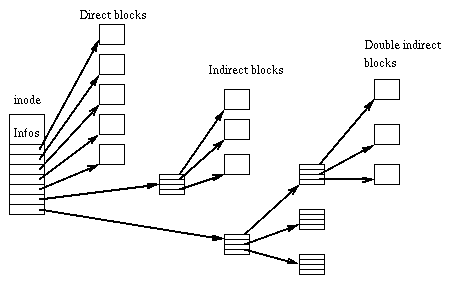
\includegraphics{./images/Ext2-inode.png}
 % Ext2-inode.png: 456x286 pixel, 96dpi, 12.06x7.57 cm, bb=0 0 342 214
\end{center}


\subsubsection{Block Groups}
En búsqueda de eficiencia y organización, ext2 divide los bloques de la partición en varios grupos.
Estos grupos tienen un número igual de bloques y de \textit{inodes}.

El objetivo principal de creación de estos, es reducir la fragmentación. 
Permiten buscar bloques disponibles para uso dentro del mismo grupo en el que se encuentra un \textit{inode}, así teniendo toda la información en bloques 
lo más cercano posibles.

En particular, estos contienen:
\begin{itemize}
\item Bitmap de uso de bloques
\item Bitmap de uso de \textit{inodes}
\item Tabla de \textit{inodes}
\item Bloques de datos
\end{itemize}

La ubicación de esta información, y otros datos sobre el uso de un dado grupo, se encuentra en la \textit{Block Group Descriptor Table}.
Esta se encuentra en el bloque inmediatamente posterior al \textit{Superblock}.
En ella se almacenan muchos datos utilizados con el objetivo de poder verificar el correcto estado del file system.

\subsubsection{Entradas de directorio}
Ext2 define como se almacena el contenido de un directorio.
Se hace de una manera muy simple en forma de \textit{Linked List}.
Cada entrada contiene un nombre, y un número de \textit{inode} al que hace referencia.
Como consecuencia, cada \textit{inode} puede ser referenciado con más de un nombre, creando lo conocido como \textit{hard links}.

\subsubsection{Limitaciones}
El tamaño máximo de la partición, y de los \textit{inodes}, es definido en función del tamaño de bloque.
Y en nuestro caso, se ve limitado por el driver ATA que soporta direccionar hasta $ 2^{28} $ sectores.

El límite teórico de tamaño total viene dado por $ 2^{32} * blockSize $.
Ahora, como nuestro driver ATA soporta solo sectores de 512 bytes, el límite real es $ 2^{28} * 512 bytes $.

El límite de tamaño de un \textit{inode} viene dado por:
$$( \frac{blockSize}{4}^3 + \frac{blockSize}{4}^2 + \frac{blockSize}{4} + 11 ) * blockSize $$

\subsection{Virtual file system}

Para proveer una interfaz desacoplada de la implementación particular de ext2, creamos el \textit{VFS}.
Este representa en memoria la estructura de \textit{inode} y \textit{File Descriptors}.
Y es el que utilizan los procesos para leer y escribir de archivos.

Este diseño nos permitió gran flexibilidad a la hora de implementar los distintos comportamientos esperados del file system.

\subsection{Apertura y manejo de archivos}
En una primera instancia nos encargamos de adaptar nuestras llamadas a sistema y nuestra librería estándar
para que puedan desarrollar las nuevas funcionalidades de nuestro sistema operativo.
Las llamadas a \textit{read} y \textit{write} podían ahora escribir en archivos, así como las llamadas a \textit{open} y \textit{close} se hicieron
necesarias cuando antes no lo fueron.
Al hacer una llamada a \textit{open()}, ésta actualizaba tanto a nivel kernel como a nivel proceso que cierto archivo habia sido abierto. 
Como ya fue dicho, un proceso contaba con una tabla de \textit{file descriptors}. 
Estos, apuntan al \textit{inode} siendo manipulado y además cuentan con punteros a función que indican como deben comportarse lecturas y escrituras (entre otras cosas) dependiendo el tipo de archivo 
(podría bien ser un archivo regular o un link simbólico por ejemplo). 
Esto permitió que las implementaciones de \textit{read()}, \textit{write()} y \textit{close()} sean bastante sencillas. 
    
Estas llamadas a sistema fueron siendo extendidas a medida que la funcionalidad del sistema operativo crecía. 
Como será visto en las próximas secciones, se escribieron funciones adecuadas para la manipulación de cada tipo de archivo.

Cabe destacar que en memoria en un dado momento existe una sola representación de un dado \textit{inode}.
Siempre que se desea pedir un \textit{inode}, si éste ya está en uso, se devuelve esa misma referencia.
Mediante \textit{Reference Counting} se asegura que solo se tenga cargados los \textit{inodes} necesarios, y que estos no se quiten de memoria antes de tiempo.

\subsection{Directorios}

Ya a bajo nivel era posible detectar el tipo de \textit{inode} guardado en el sistema. Un directorio simplemente era
un \textit{inode} en cuyo contenido se guardan referencias hacía otros \textit{inodes}. Tanto la interfaz del driver Ext2 como la del
vfs permiten escribir directorios de forma correcta. Cabe destacar que además de la referencia al \textit{inode}, una entrada
de directorio también guarda el nombre de la entrada que luego verá el usuario.

\subsection{FIFO}
La implementación de \textit{FIFOs} resultó trivial, ya que muchas de las decisiones diseño tomadas antes de implementarlos los tenían en cuenta.
La existencia de la estructura \textit{FileDescriptorOps} que contiene punteros a función con las operaciones realizables sobre un File Descriptor,
 permitió que la implementación sea totalmente transparente a nivel sistema.

Al \textit{inode} que representa un FIFO, cuando es abierto por primera vez se le asocia una estructura \textit{FIFO}.
Como todos los File Descriptors que representan un mismo archivo hacen referencia al mismo \textit{inode}, todos tiene acceso la estructura \textit{FIFO}.
Esta contiene el buffer donde se guardan los datos escritos al FIFO, cuantos procesos abrieron el fifo, y otro datos útiles.

Cabe destacar el comportamiento de los FIFOs en cuanto su apertura, estrictura y lectura.
Cuando se abre un FIFO, el proceso se bloquea hasta que el FIFO es abierto por al menos un proceso para lectura, y otro para escritura.
La lectura de un FIFO es bloqueante, es decir si no hay contenido para leer, el proceso bloquea hasta que lo haya.
De la misma manera, la escritura es bloqueante, en caso de que el FIFO no tenga espacio para escribir los datos.

En caso de que alguna punta del FIFO sea cerrada por todos los procesos que la abrieron, cualquier operación en curso se cancela, y retorna que se procesaron 0 bytes.

\subsection{Links simbólicos}
La implementación de links simbólicos implicaba la creación de nodos que inclusive en el sistema Ext2 eran marcados
como links simbólicos. El contenido de los mismos simplemente indicaba el \textit{path} del archivo al que este
hacia referencia.
Luego, a la hora de leer un archivo que sea un link simbolico (o al tratar de resolver un \textit{path} en el que alguno
de sus directorios era un link simbólico) bastaba con reemplazar este link con el archivo al que realmente
apuntaba.

En esta implementación (al igual que en el resto) tratamos de ser lo más fieles al entorno \textit{UNIX} como nos fue posible.

\subsection{Character devices}
Para nuestra implementación de \textit{tty}, usamos el tipo especial de archivos \textit{Character device}.
Esto quiere decir que toda la comunicación entre la terminal y los procesos corriendo en ella, pasa a través del \textit{VFS}.

\subsection{Current working directory}
    
Como ya fue mencionado, cada proceso contiene información sobre cual era el \textit{current working directory} en
el momento en que fue ejecutado. Esto permite que la obtención del \textit{current working directory} sea sencilla
y manipulable en los momentos necesarios, sobre todo para permitir \textit{paths} relativos.

    
\subsection{Permisos del sistema}
Una vez implementados usuarios y grupos fue fácil saber el gid y el uid de un proceso. Dada la forma en que estaba
implementado nuestro \textit{file system}, Ext2 contaba con lugares específicos para guardar tanto los permisos y el
uid y gid del archivo. Además, las prestaciones del vfs hacían que estos datos también fuesen fáciles de obtener.

Una vez conseguidos estos datos, era trivial evaluar en que casos se permitía abrir un archivo, teniendo en cuenta
que tanto el archivo tenga los permisos adecuados así como el \textit{path} que lo contiene.

\newpage
\section{Comandos provistos}
Para poder probar y mostrar las nuevas funcionalidades del trabajo hubo que agregar ciertos comandos y funcionalidades ejecutables desde la consola. 
La lista completa de comandos disponibles puede encontrarse mediante el comando \textit{help}, y la documentación de cada comando mediante el comando \textit{man}.


A continuación se presentan algunos casos interesantes.

\newpage
\section{Agregados}
\subsection{Memory managment}
Inicialmente, el TP contaba con múltiples arrays de tamaño estático para guardar todos los datos internos del kernel.
Por supuesto, esta solución es menos que óptima, ya que genera un desperdicio de memoria e impone límites arbitrarios al sistema.
Para evitar esto, desarrollamos un sistema de allocación de páginas de memoria.
Y encima de este sistema, utilizamos la implementación de \textit{malloc} de Dario Sneidermanis, publicada en \href{https://github.com/esneider/malloc}{Github}.

Para allocar páginas, hicimos uso de información provista por \textit{Grub} que permite saber exactamente qué zonas de memoria se pueden utilizar, 
y cuanta memoria hay disponible.
Esta memoria la dividimos en bloques de $4KB$, teniendo en mente la posibilidad de agregar paginación al sistema.
Para obtener estas páginas optamos por un simple algoritmo de allocación basado en un bitmap de uso de páginas.

Una característica interesante de la implementación de \textit{malloc}, es que permite tener varios contextos de memoria distintos.
Lo que facilitó tener un contexto de memoria para el kernel, y otro para cada proceso (excepto los procesos de kernel que usan el mismo que el kernel).
La única limitación del sistema es que los contextos de proceso tienen un tamaño fijo, mientras que el del kernel crece a medida que es necesario.

\subsection{Terminal control sequences}
Nuestra implementación de terminal soporta una gran parte de \href{http://invisible-island.net/xterm/ctlseqs/ctlseqs.html}{xterm control sequences}.
Estas permiten manipular el cursor y el color de la pantalla desde los procesos utilizando sólo la primitiva \textit{write}.

\newpage
\section{Problemas encontrados}

Durante el desarrollo de este trabajo práctico fueron surgiendo diferentes dudas y problemas. El propósito de esta
sección es comentarlos con el fin reflejar proceso de aprendizaje.

Un dilema bastante frecuente a lo largo del trabajo práctico fue lo que nos gusta llamar el problema de ``la gallina o el huevo''. Al realizar
un desarrollo a bajo nivel que ha comenzado con pocos recursos, era habitual encontrarse con la duda de si convenía
arrancar a implementar la lectura o la escritura de alguna prestación. Es evidente que si se hacía primero la lectura, 
no había forma de probar su funcionamiento ya que no existía la escritura. Lo mismo sucedía a modo inverso. Si bien 
la solución no era complicada (desarrollar todo) era incómodo y molesto a la hora de encontrar errores ya que los mismos
podían encontrarse en cualquier lado.

Varios problemas interesantes surgieron durante la creación del \textit{driver} ATA. A pesar de que se siguieron
rigurosamente los estándares, se encontró que no todos los emuladores funcionaban de forma correcta con el mismo.
Inclusive, detectamos que el driver no se comportaba de manera deseada al tratar con varios sectores a la vez con lo
cual nos vimos forzados a modificar la lógica interna del driver simulando un acceso a múltiples sectores a tráves de
varios accesos de a un sector a la vez.


<<<< Mencionar el tema de los comandos internos de la shell >>>>

\newpage     
\section{Referencias}

\begin{itemize}
  \item Material provisto por la cátedra
  \item The C programming language - Kernighan y Ritchie
  \item http://invisible-island.net/xterm/ctlseqs/ctlseqs.html
  \item http://webpages.charter.net/danrollins/techhelp/0087.HTM
  \item http://faydoc.tripod.com/cpu/rdtsc.htm
  \item http://stanislavs.org/helppc/
  \item http://www.linux.it/~rubini/docs/ksys/ksys.html
  \item http://wiki.osdev.org
  \item http://wiki.osdev.org/Detecting\_CPU\_Speed
  \item	http://wiki.osdev.org/CMOS\#Accessing\_CMOS\_Registers
  \item http://wiki.osdev.org/Bootable\_CD
  \item http://wiki.osdev.org/Boot\_sequence\#Easy\_Way\_Out
  \item http://wiki.osdev.org/Ext2
  \item http://wiki.osdev.org/IDE
  \item http://wiki.osdev.org/ATA\_PIO\_Mode
  \item http://en.wikipedia.org/wiki/System\_time\#Retrieving\_system\_time
  \item http://en.wikipedia.org/wiki/Calculating\_the\_day\_of\_the\_week
  \item http://cplusplus.com/
  \item http://github.com/esneider/malloc
  \item http://www.nongnu.org/ext2-doc/ext2.html
\end{itemize}
   
\end{document}
